\chapter{Implementation}
\section{Platform}
We choose a C++ language for implementing our solutions, because we need low level code optimization and features like SIMD instructions, which are not available in other languages. Even if the CUDA is developed to work with multiple languages, cooperation with  C++ is one of the best, because also CUDA kernels are written in C++. Also platform independence of C++ is useful because we developed programs on Windows and than run on Linux clusters.

\section{K-means algorithm} \label{sec:kMeansAlgorithm}
We focused on standard k-means algorithm~\cite{hartigan1979algorithm}, which input is set of $n$ points in $d$-dimensional space $R^d$ and an number of centroids $k$. The task is to assign points to centroids and minimize the distance between points and centroids. Algorithm works iteratively and each iteration consist of two steps. At first points are assigned to the nearest centroids and than new centroids are computed. Algorithm ends after known number of steps or when nothing changes between two iterations. Output of the this algorithm are centroids coordinates or points with assigned clusters.\\
As we can see in serial implementation~\autoref{lst:kMeansCode}, there are many cycles dependent on data size, so with growing number of data, serial version comes much slower. For example in two nested cycles on lines \autoref{lst:nestedCyclesBegin}-\autoref{lst:nestedCyclesEnd} of \autoref{lst:kMeansCode}, slowdown is great and this part of code is good target for parallelization.\\

\begin{lstlisting}[caption={k-means algorithm}, language=C++, escapeinside={\%*}{*)}, label={lst:kMeansCode}, numbers=left]
CreateLSH(width, hashTablesCount, basicHashFunctions)
{
  // Main iteration loop
  for( i = 0; i < iterationsCount; i++)
  {
    assign_to_clusters(data, means);
    compute_means(data_means);
  }
}

// Assign points to clusters
%*\label{lst:assignToClusters}*)assign_to_clusters(data, means)
{
//Iterate through data
%*\label{lst:nestedCyclesBegin}*)  for( d = 0; d < data_size; d++)
  {
    assigned_cluster = 0;
    min_distance = MAX_VALUE;
// Iterate through means
    for( m = 0; m < means_size; m++)
    {
      distance = count_distance( data[d], means[m] );
// If m-cluster is closer, reassign cluster
      if ( distance < min_distance )
      {
        assigned_cluster = m;
        min_distance = distance;
      }
    }
    data[d]->assigned_cluster = assigned_cluster;
%*\label{lst:nestedCyclesEnd}*)  }
}

// Compute new means
%*\label{lst:computeNewMeans}*)compute_means(data, means)
{
// Create new means array, all values are set to 0
  for( m = 0; m < means_size; m++)
  {
    new_means.push_back(new mean(0));
  }
  
// Iterate through data and accumulate data in appropriate new mean
  for( d = 0; d < data_size; d++)
  {
    assigned_cluster = data[d]->assigned_cluster;
    new_means[assigned_cluster]->contained_points++;
    for( dim = 0; dim < dimensions; dim++)
    {
      new_means[assigned_cluster]->coordinates[dim] +=
        data[d]->coordinates[dim];
    }
  }
  
// Count new means coordinates (arithmetic mean)
  for( m = 0; m < means_size; m++)
  {
    for( dim = 0; dim < dimensions; dim++)
    {
      new_means[m]->coordinates[dim] /=
        new_means[m]->contained_points;
    }
  }
}

// Function for counting distance
count_distance(point, mean)
{
  sum_squares = 0;
  for( dim = 0; dim < dimensions; dim++)
  {
    difference = point->coordinates[dim] - mean->coordinates[dim];
    sum_squares += difference * difference;
  }
  return sqrt( sum_squares );
}
\end{lstlisting}

\section{Parallelization}
As we mentioned in \autoref{sec:kMeansAlgorithm}, classical k-means algorithm contains many compute-intensive cycles, which could be parallelized. Problem is that the algorithm contains some compute dependencies, for example parallelization of nested cycles on lines \autoref{lst:nestedCyclesBegin}-\autoref{lst:nestedCyclesEnd} of \autoref{lst:kMeansCode} is problematic, because we need to accumulate coordinates in shared variable. These dependencies must be solved some way for correct parallelization.

\subsection{CPU versions}
We tried to used the most modern technologies offered by the newest CPU architectures to speed up k-means algorithm by parallelization. We created two levels of parallelization, first based on thread level (using more logical cores on single CPU) and than vectorization level using SIMD instructions.

\subsubsection{Thread level parallelization}
For thread level parallelization, we choose Threading Building Blocks (TBB) library from Intel. This library offers algorithms and data structures for parallel programing using multi-core processors but relieve programmer from complications arising from the use of native threading packages and handling particular threads. Manual thread creation, execution, synchronization and termination is hidden by using by creating TBB tasks which are processed on individual cores dynamically by the library. Also efficient use of CPU caches is automated.\\
We reworked program so points are split in groups, each group forming one TBB task.\\
\begin{description}
\item[Assigning to clusters]The first part of algorithm, assigning to clusters~\autoref{lst:kMeansCode},~\autoref{lst:assignToClusters}, is not so problematic, because only write operation is assigning cluster to point. Each point is contained in one and only one TBB task, which is processed by single thread, so it could not be read or written from other threads.\\
Second possible solution is to split means into groups and parallelize algorithm by tasks containing means. This solution is significantly slower, because we must synchronize writing information to each point about assigned cluster. If we want to remember this information in means (by accumulating assigned points to each mean) we hit a problem, because after assigning point to mean, we could not know if other mean is not closer to processed point so this way o parallelization is too computationally intensive.\\
\item[Compute new means]The second part of the algorithm, counting new means~\autoref{lst:kMeansCode},~\autoref{lst:computeNewMeans}, is more problematic, because we approach means from different TBB tasks, so accumulating of coordinates must be synchronized. We solved this problem by local copy of means in each TBB task, so we avoided the collisions. For joining tasks, we used TBB reduce algorithm, when to tasks are joined, local arrays of means coordinate sums are correctly added.\\
Also in this part of algorithm exists second possible solution by approaching parallelization by splitting means. This is more compute intensive because in this solution, for each mean, we must iterate through all points and accumulate coordinates but in previous solution, we iterate only through points and than, we join single tasks which takes logarithmic time depends on number of tasks.
\end{description}
Because both tasks are parallelized by same approach (splitting points to tasks, not the means), we joined both steps into one~\autoref{fig:computeflow} and gain more speed up because of omitting one start and one finish of TBB parallel task which has big overhead.
\begin{figure}[h]
  \centering
  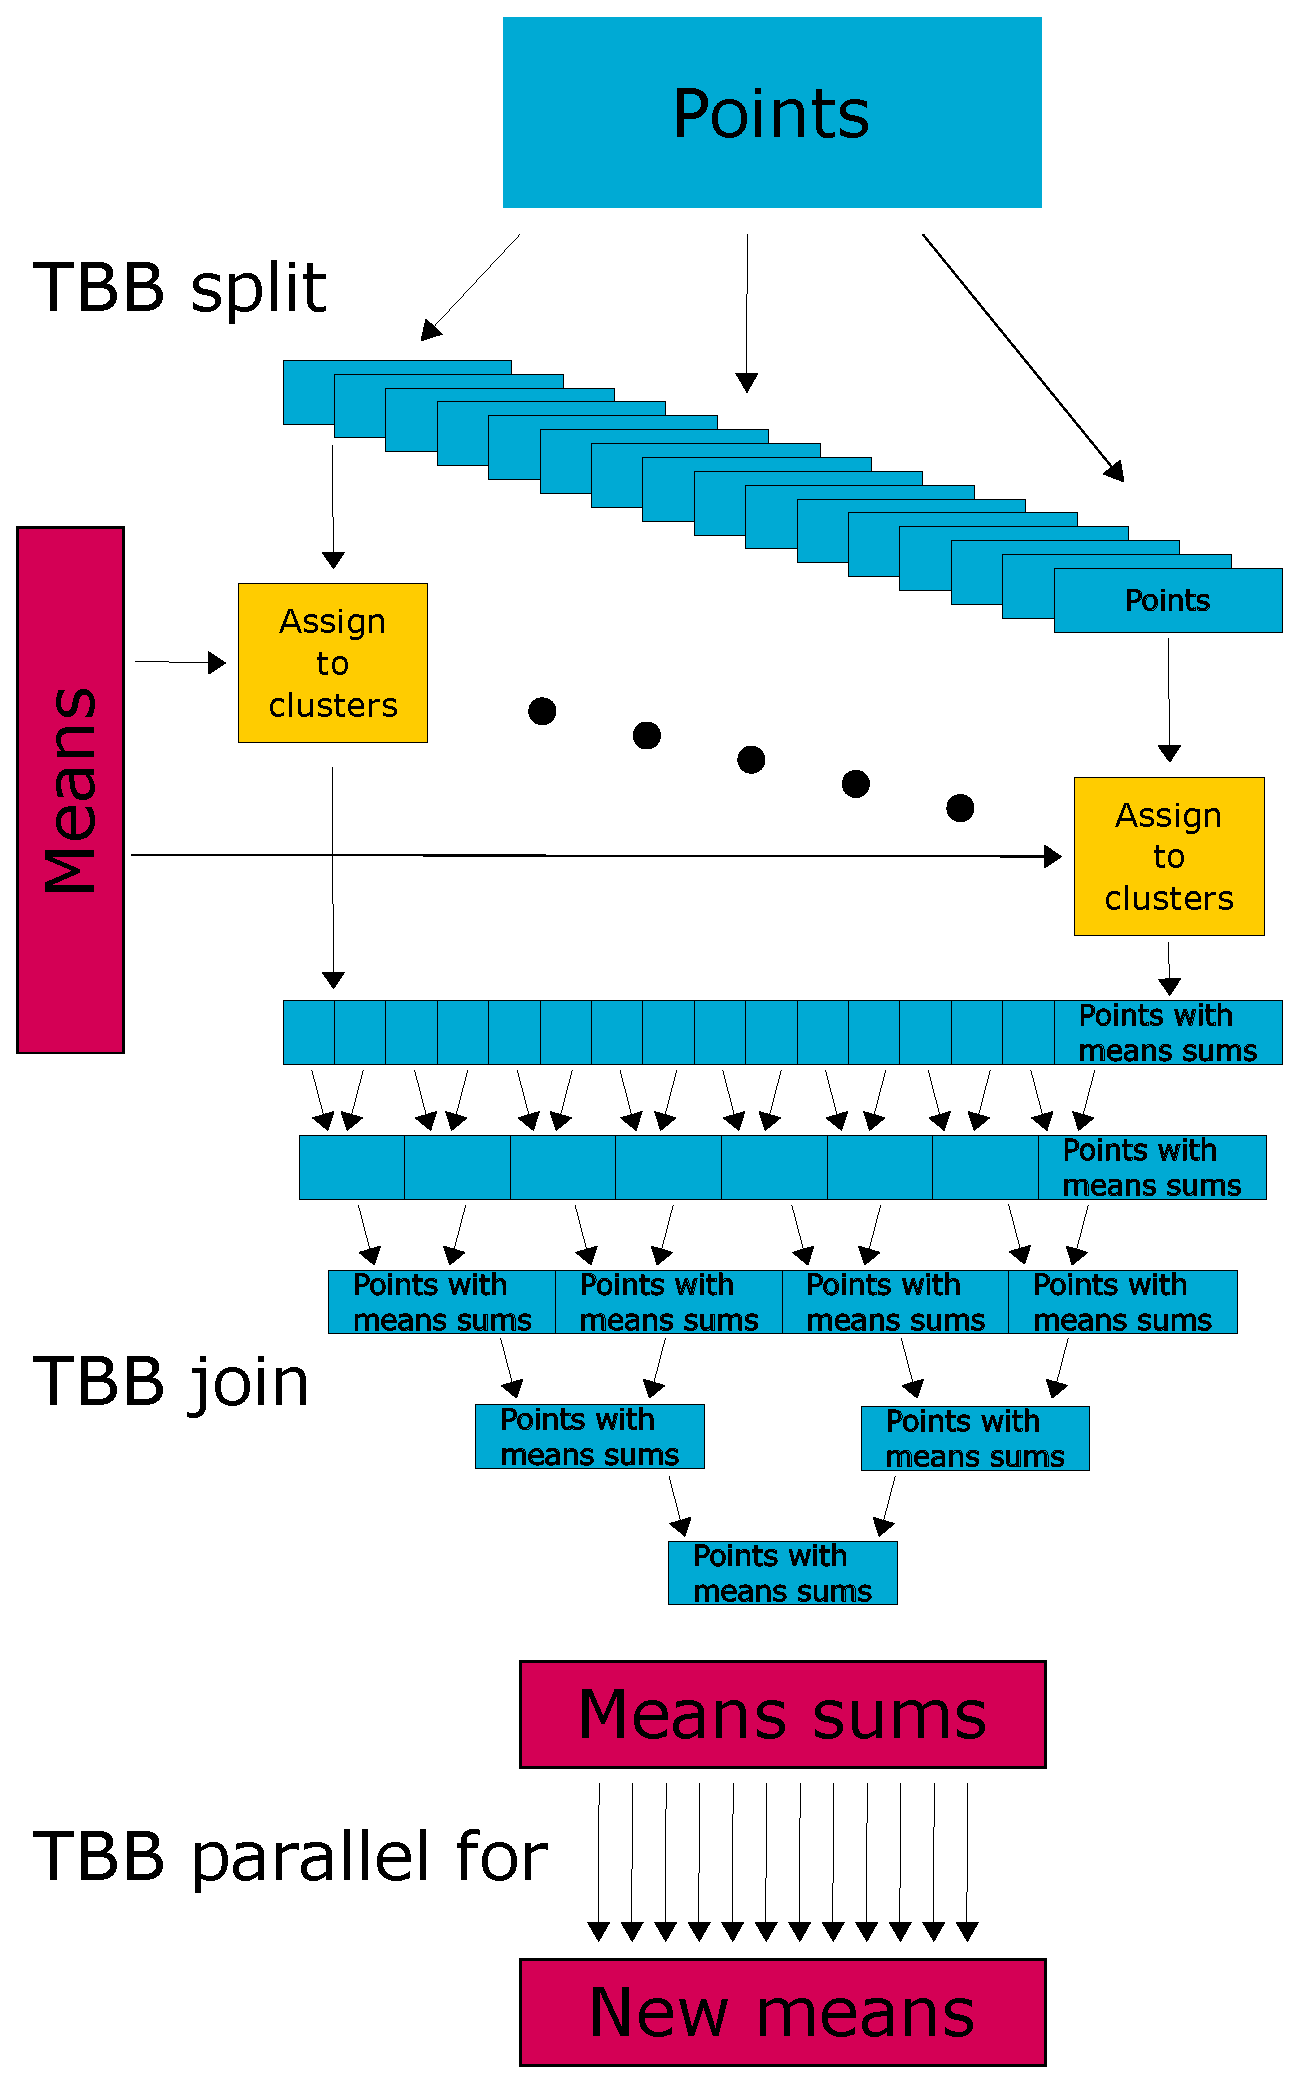
\includegraphics[width=1\linewidth]{img/computeFlow.eps}
  \caption{Compute flow}
  \label{fig:computeflow}
\end{figure}
\subsubsection{Vectorization}
For additional speed-up, we decided to use Simple instruction, multiple data (SIMD) as second layer of parallelization, concretely Streaming SIMD instructions (SSE), which are extension of x86 architecture. These instructions could greatly speed up the computation when exactly the same operations are performed on multiple data objects. Because points are already parallelized by TBB, we use SIMD inductions to parallelize smaller cycles iterating through dimensions, which are very often used in the algorithm. This cycle is usually much smaller (up to number of dimensions) than data but contains only few instructions which is precisely suitable for usage of SSE instructions so the loops will be up to four times faster (depend on number of dimensions) than non-SSE version.
\subsection{GPU versions}
For maximum speedup of this algorithm, we implemented versions using GPU, which offers hundreds of cores, so speed up of algorithm should be more than ten times better than parallel CPU version. Because of GPU architecture special features and the wide diversity of the input data, we developed more algorithm versions to reflect this particularities.\\
Because the GPU compute effectiveness very depends on using different types of memory and the efficiency of its usage, it really depends on algorithm design. This problem is difficult to solve by single algorithm, because we need to use the data input characteristics, which could be the following:
\begin{description}
\item[Many dimensions]
\item[Few means]
\item[Big data]
\end{description}

% TOTO add table dataSize x memory fit
\section{Tools}